\documentclass[12pt]{article}
%\usepackage[document]{ragged2e}
\usepackage{array, amssymb, amsthm, linguex, enumerate, amsmath, physics, enumitem, xcolor, graphicx, xparse}
\let\fg\undefined %remove linguex/siunitx naming clash
\usepackage[english]{babel}
\usepackage[letterpaper,top=2cm,bottom=2cm,left=3cm,right=3cm,marginparwidth=1.75cm]{geometry}
\usepackage[colorlinks=true, allcolors=blue]{hyperref}
\usepackage[group-separator={,}]{siunitx} %\num{12345} -> "12,345"
\usepackage{fancyhdr}
\usepackage{notomath}
\usepackage[T1]{fontenc}
\usepackage{multicol}
\usepackage{mathtools}

%Number sets
\newcommand{\R}{\mathbb{R}}
\newcommand{\C}{\mathbb{C}}
\newcommand{\N}{\mathbb{N}}
\newcommand{\F}{\mathbb{F}}
\renewcommand{\Re}{\operatorname{Re}}
\renewcommand{\Im}{\operatorname{Im}}
\renewcommand{\L}[1]{\mathcal{L}\left({#1}\right)} %Linear Map

\newcommand{\pmp}{\,\pm\,} %add small extra space to \pm

\NewDocumentCommand{\ceil}{ s m }{% ceiling brackets
    \IfBooleanTF{#1}%
    {\lceil #2 \rceil}% starred: no-autosizing
    {\left\lceil #2 \right\rceil}% unstarred: autosizing
}

\NewDocumentCommand{\ceiling}{ s m }{% ceiling brackets
    \IfBooleanTF{#1}%
    {\lceil #2 \rceil}% starred: no-autosizing
    {\left\lceil #2 \right\rceil}% unstarred: autosizing
}

\NewDocumentCommand{\floor}{ s m }{% floor brackets
    \IfBooleanTF{#1}%
    {\lfloor #2 \rfloor}% starred: no-autosizing
    {\left\lfloor #2 \right\rfloor}% unstarred: autosizing
}

\NewDocumentCommand{\pars}{ s m }{% parenthesis
    \IfBooleanTF{#1}%
    {( #2 ) }% starred: no-autosizing
    {\left( #2 \right) }% unstarred: autosizing
}

\NewDocumentCommand{\inner}{ s m }{% inner product
    \IfBooleanTF{#1}%
    {\langle #2 \rangle}% starred: no-autosizing
    {\left\langle #2 \right\rangle}% unstarred: autosizing
}

\NewDocumentCommand{\innerconj}{ s m }{% inner product
    \IfBooleanTF{#1}%
    {\overline{\langle #2 \rangle}}% starred: no-autosizing
    {\overline{\left\langle #2 \right\rangle}}% unstarred: autosizing
}

\NewDocumentCommand{\brac}{ s m }{% brackets
    \IfBooleanTF{#1}%
    {[#2] }% starred: no-autosizing
    {\left[ #2 \right] }% unstarred: autosizing
}

%default latex bracket size naming
\newcommand{\biggbrac}[1]{\bigg[ {#1} \bigg] }
\newcommand{\bigbrac}[1]{\big[ {#1} \big] }
\newcommand{\Bigbrac}[1]{\Big[ {#1} \Big] }


\RenewDocumentCommand{\over}{ s m }{% fraction 1/arg
    \IfBooleanTF{#1}%
    {\dfrac{1}{#2}}% starred: dfrac
    {\frac{1}{#2}}% unstarred: normal frac
}

\NewDocumentCommand{\pover}{ s m }{% parenthesis around fraction (1/arg)
    \IfBooleanTF{#1}%
    {\left(\dfrac{1}{#2}\right)}% starred: dfrac
    {\left(\frac{1}{#2}\right)}% unstarred: normal frac
}

\NewDocumentCommand{\pfrac}{ s m m}{% parenthesis around fraction (arg1/arg2)
    \IfBooleanTF{#1}%
    {\left( \dfrac{{#2}}{{#3}} \right)}% starred: dfrac
    {\left( \frac{{#2}}{{#3}} \right)}% unstarred: normal frac
}


\newcommand{\Xbar}{\bar{X}}
\newcommand{\Ybar}{\bar{Y}}
\newcommand{\xbar}{\bar{x}}
\newcommand{\ybar}{\bar{y}}

\newcommand{\symint}[1]{\int_{- #1}^{#1}}

\newcommand{\limn}{\lim_{n\to\infty}}

\newcommand{\sumn}[1]{\sum_{n=#1}^{\infty}}

\newcommand{\nptl}{\frac{n \pi t}{L}}
\newcommand{\npt}{n \pi t}
\newcommand{\npto}[1]{\frac{n \pi t}{#1}}

\newcommand{\npxl}{\frac{n \pi x}{L}}
\newcommand{\bnxl}{\frac{\beta_n x}{L}}
\newcommand{\npx}{n \pi x}
\newcommand{\np}{n \pi}
\newcommand{\npxo}[1]{\frac{n \pi x}{#1}}
\newcommand{\onp}[1]{\frac{#1}{n \pi}}
\newcommand{\onps}[1]{\frac{#1}{n^2 \pi^2}}
\newcommand{\onpc}[1]{\frac{#1}{n^3 \pi^3}}
\newcommand{\npo}[1]{\frac{n \pi}{#1}}
\newcommand{\cosp}[1]{\cos \pars{#1}}
\newcommand{\sinp}[1]{\sin \pars{#1}}
\newcommand{\intll}{\int_{-L}^{L}}
\newcommand{\intl}{\int_{0}^L}

\newcommand{\gammaDist}[2]{\operatorname{Gamma} \left( {#1},{#2} \right)} %gamma distribution
\NewDocumentCommand{\normalDist}{s g g}{ %normal distibution
    \IfBooleanTF{#1} { % starred, no autosizing parenthesis
      \IfNoValueTF{#2}{
          N (\mu,\, \sigma^2 ) %\normalDist* "default" normal distribution N(\mu, \sigma^2)
        } {
            \IfNoValueTF{#3}{N (#2)}{} %\normalDist{arg} --> N(arg)
        }
      \IfNoValueTF{#3}{}{N ( #2, #3 )}  %\normalDist*{arg1}{arg2} --> N(arg1,arg2)
    }  % else (unstarred) autosize parenthesis
    {
        \IfNoValueTF{#2}{
            N \left(\mu,\, \sigma^2 \right) %\normalDist "default" normal distribution N(\mu, \sigma^2)
        } {
            \IfNoValueTF{#3}{N \left(#2\right)}{} %\normalDist{arg} --> N(arg)
        }
        \IfNoValueTF{#3}{}{N \left( #2, #3 \right)} %\normalDist{arg1}{arg2} --> N(arg1,arg2)
    }
}



%colors
\definecolor{ggreen}{RGB}{0, 127, 0}
\definecolor{dgray}{RGB}{63,63,63}
\definecolor{neonorange}{RGB}{255,47,0}
\definecolor{mygray}{rgb}{0.5,0.5,0.5}
\definecolor{eblue}{RGB}{0,74,127}
\newcommand{\red}[1]{\color{red}{#1}\color{black}}
\newcommand{\green}[1]{\color{ggreen}{#1}\color{black}}
\newcommand{\blue}[1]{\color{blue}{#1}\color{black}}
\newcommand{\setRed}{\color{red}}
\newcommand{\setBlack}{\color{black}}
\newcommand{\setBlue}{\color{blue}}
\newcommand{\setGreen}{\color{ggreen}}

\newcommand{\coshp}[1]{\cosh \pars{#1}}
\newcommand{\sinhp}[1]{\sinh \pars{#1}}
\newcommand{\cunt}{\frac{c n \pi t}{L}}
\newcommand{\absl}{\abs{\lambda}}
\newcommand{\rabsl}{\sqrt{\abs{\lambda}}}
\newcommand{\qiffq}{\quad\iff\quad}
\newcommand{\thru}[1]{{#1}_1, \dots, {#1}_n}
\newcommand{\sumThru}[1]{{#1}_1 + \cdots + {#1}_n}
\newcommand{\yn}{Y_1, \dots, Y_n} % Y_1, ..., Y_n
\newcommand{\xn}{X_1, \dots, X_n} % Y_1, ..., Y_n

%hats and tildes
\newcommand{\that}{\widehat{\theta}} % theta hat
\newcommand{\phat}{\widehat{p}} % p hat
\newcommand{\qhat}{\widehat{q}} % p hat
\newcommand{\psihat}{\widehat{\psi}} % psi hat
\newcommand{\Psihat}{\widehat{\Psi}} % Psi hat
\newcommand{\ptilde}{\widetilde{p}} % psi tilde
\newcommand{\Psitil}{\widetilde{\Psi}} % Psi tilde
\newcommand{\betah}{\widehat{\beta}} % beta hat

%2x2 matrix shortcuts
\newcommand{\detx}[4]{\begin{vmatrix}{#1} & {#2}\\{#3}&{#4}\end{vmatrix}} % 2x2 determinant
\newcommand{\dety}[9]{\begin{vmatrix}{#1} & {#2} & {#3} \\{#4}&{#5}&{#6}\\ {#7} & {#8} & {#9}\end{vmatrix}} % 3x3 determinant
\newcommand{\bmaty}[9]{\begin{bmatrix}{#1} & {#2} & {#3} \\{#4}&{#5}&{#6}\\ {#7} & {#8} & {#9}\end{bmatrix}} % 3x3 matrix
\newcommand{\bmat}[4]{\begin{bmatrix}{#1} & {#2}\\{#3}&{#4}\end{bmatrix}} % 2x2 matrix brackets
\renewcommand{\pmat}[4]{\begin{pmatrix}{#1} & {#2}\\{#3}&{#4}\end{pmatrix}} % 2x2 matrix parenthesis

%remove any enumerate/itemize indent temporarily
\makeatletter   %% <- make @ usable in macro names
\newcommand*\notab[1]{%
  \begingroup   %% <- limit scope of the following changes
    \par        %% <- start a new paragraph
    \@totalleftmargin=0pt \linewidth=\columnwidth
    %% ^^ let other commands know that the margins have been reset
    \parshape 0
    %% ^^ reset the margins
    #1\par      %% <- insert #1 and end this paragraph
  \endgroup
}
\makeatother    %% <- revert @


\newcommand{\dimrange}[1]{\operatorname{dim}\operatorname{range}{#1}} % dimrange
\newcommand{\dimnull}[1]{\operatorname{dim}\operatorname{null}{#1}} % dimnull
\newcommand{\range}[1]{\operatorname{range}{#1}} %range
\newcommand{\nullspace}{\operatorname{null}} %null

% polynomial notation
\NewDocumentCommand{\poly}{ s g g }{%
    \IfBooleanTF{#1} {
        \IfNoValueTF{#2} {
            \mathcal{P}(\mathbb{R})
        } {
            \mathcal{P}_{#2}(\mathbb{R})
        }
    } {
        \IfNoValueTF{#3} {
            {\mathcal{P}(#2)}
        } { %else
            {\mathcal{P}_{#2}(#3)}
        }
    }
}

\NewDocumentCommand{\bias}{ s m }{% bias(arg)
    \IfBooleanTF{#1}%
    {\operatorname{bias}(#2)}% starred: no autosizing
    {\operatorname{bias}\left(#2\right)}% unstarred: autosizing
}

\NewDocumentCommand{\MSE}{ s m }{% MSE(arg)
    \IfBooleanTF{#1}%
    {\operatorname{MSE}(#2)}% starred: no autosizing
    {\operatorname{MSE}\left(#2\right)}% unstarred: autosizing
}

\NewDocumentCommand{\Var}{ s m }{% variance with parenthesis V(arg)
    \IfBooleanTF{#1}%
    {\operatorname{Var}(#2)}% starred: no autosizing
    {\operatorname{Var}\left(#2\right)}% unstarred: autosizing
}

\NewDocumentCommand{\Varb}{ s m }{% variance with brackets V[arg]
    \IfBooleanTF{#1}%
    {\operatorname{Var}[\,#2\,]}% starred: no autosizing
    {\operatorname{Var}\left[\,#2\,\right]}% unstarred: has autosizing
}

\NewDocumentCommand{\Vb}{ s m }{% another renaming of variance with brackets V[arg]
    \IfBooleanTF{#1}%
    {\operatorname{Var}[\,#2\,]}% starred: no autosizing
    {\operatorname{Var}\left[\,#2\,\right]}% unstarred: has autosizing
}

\NewDocumentCommand{\E}{ s m }{% expectation with parenthesis E(arg)
    \IfBooleanTF{#1}%
    {\operatorname{E}(#2)}% starred: no autosizing
    {\operatorname{E}\left(#2\right)}% unstarred: has autosizing
}

\NewDocumentCommand{\Eb}{ s m }{% expectation with brackets E[arg]
    \IfBooleanTF{#1}%
    {\operatorname{E}[#2]}% starred: no autosizing
    {\operatorname{E}\left[#2\right]}% unstarred: has autosizing
}

\RenewDocumentCommand{\P}{ s m }{% probability with parenthesis Pr(arg)
    \IfBooleanTF{#1}%
    {\Pr (#2) }% starred: no autosizing
    {\Pr \left( #2 \right) }% unstarred: has autosizing
}

\NewDocumentCommand{\prob}{ s m }{% probability with parenthesis Pr(arg)
    \IfBooleanTF{#1}%
    {\Pr (#2) }% starred: no autosizing
    {\Pr \left( #2 \right) }% unstarred: has autosizing
}

\NewDocumentCommand{\eff}{ s m }{% efficiency with parenthesis eff(arg)
    \IfBooleanTF{#1}%
    {\operatorname{eff}(#2)}% starred: no autosizing
    {\operatorname{eff}\left(#2\right)}% unstarred: has autosizing
}

%vertical vector of up to 8 elements
\NewDocumentCommand\vvec{s m g g g g g g g}{%
    \IfBooleanTF{#1} {
        \begin{bmatrix}% if starred use brackets
            \IfNoValueTF{#2}{}{#2}
            \IfNoValueTF{#3}{}{\\#3}
            \IfNoValueTF{#4}{}{\\#4}
            \IfNoValueTF{#5}{}{\\#5}
            \IfNoValueTF{#6}{}{\\#6}
            \IfNoValueTF{#7}{}{\\#7}
            \IfNoValueTF{#8}{}{\\#8}
        \end{bmatrix}
    }  % else (unstarred) use parethesis
    {
        \begin{pmatrix}%
            \IfNoValueTF{#2}{}{#2}
            \IfNoValueTF{#3}{}{\\#3}
            \IfNoValueTF{#4}{}{\\#4}
            \IfNoValueTF{#5}{}{\\#5}
            \IfNoValueTF{#6}{}{\\#6}
            \IfNoValueTF{#7}{}{\\#7}
            \IfNoValueTF{#8}{}{\\#8}
        \end{pmatrix}
    }
}
\def\Cov{\operatorname{Cov}} %Covariance
\def\df{\text{df}} %degrees of freedom

\NewDocumentCommand{\example}{ s g }{% Example header
    \IfBooleanTF{#1}%
    {\vspace{0.1in}}% starred: 0.1in
    {\vspace{0.2in}}% unstarred: 0.2in
    \IfNoValueTF{#2} {\noindent\textbf{\color{eblue} Example: }}{\noindent\textbf{\color{eblue} Example (#2): }}
}
\NewDocumentCommand{\disc}{ s }{% Discussion header
    \IfBooleanTF{#1}%
    {\vspace{0.1in}\noindent\textbf{Discussion: } }% starred: 0.1in
    {\vspace{0.2in}\noindent\textbf{Discussion: } }% unstarred: 0.2in
}
\NewDocumentCommand{\defn}{ s }{% Definition header
    \IfBooleanTF{#1}%
    {\vspace{0.1in}\noindent\textbf{\color{neonorange} Definition: } }% starred: 0.1in
    {\vspace{0.2in}\noindent\textbf{\color{neonorange} Definition: } }% unstarred: 0.2in
}
\NewDocumentCommand{\reason}{ s }{% Reason header
    \IfBooleanTF{#1}%
    {\vspace{0.1in}\noindent\textbf{Reason:} }% starred: 0.1in
    {\vspace{0.2in}\noindent\textbf{Reason:} }% unstarred: 0.2in
}
\NewDocumentCommand{\recall}{ s }{% Recall header
    \IfBooleanTF{#1}%
    {\vspace{0.1in}\noindent\textit{Recall:} }% starred: 0.1in
    {\vspace{0.2in}\noindent\textit{Recall:} }% unstarred: 0.2in
}
\NewDocumentCommand{\remark}{ s }{% Remark header
    \IfBooleanTF{#1}%
    {\vspace{0.1in}\noindent\textit{Remark:} }% starred: 0.1in
    {\vspace{0.2in}\noindent\textit{Remark:} }% unstarred: 0.2in
}

\NewDocumentCommand{\soln}{ s }{% Remark header
    \IfBooleanTF{#1}%
    {\vspace{0.1in}\noindent\textbf{Solution: } }% starred: 0.1in
    {\vspace{0.2in}\noindent\textbf{Solution: } }% unstarred: 0.2in
}

\newcommand{\proj}[2]{\operatorname{proj}_{{#1}}{#2}} %projection
\newcommand{\wideand}{\qquad \text{and} \qquad}

\newcommand{\bu}[1]{\textbf{\underline{{#1}}} } %bold underline
\newcommand{\boldit}[1]{\textbf{\textit{{#1}}} } %bold italix

% put actual quotation marks "around something"
\newcommand{\say}[1]{\textquotedblleft{#1}\textquotedblright}

% max{arg} and min{arg}
\renewcommand{\max}[1]{\operatorname{max}\left\{ #1 \right\}}
\renewcommand{\min}[1]{\operatorname{min}\left\{ #1 \right\}}

\newcommand{\Span}[1]{\operatorname{span}\left\{ #1 \right\}}

%Create a new vspace line no indent
\newcommand{\nl}{\vspace{0.1in}\noindent}
\newcommand{\nnl}{\vspace{0.2in}\noindent}
\newcommand{\nnnl}{\vspace{0.3in}\noindent}
\textwidth=7.02in
\hoffset=-.425in

\setcounter{MaxMatrixCols}{20}
\begin{document}
\pagestyle{fancy}
\fancyhf{}
\fancyhead[RO]{Matthew Wilder}
\fancyhead[LO]{MTH 427 - Homework \#7}
\fancyfoot[CO]{Page \thepage}

\noindent MTH 427 - Spring 2023
\\Assignment \#7
\\Due: Monday, 4 17 2023

\section{Exercise text book, Shumway and Stoffer}

\nnl\textbf{Problem \#2.6}
Consider a process consisting of a linear trend with an additive noise term
consisting of independent random variables wt with zero means and variances
$\sigma_w^2$, that is,
$$x_t = \beta_0 + \beta_1 t + w_t$$
where $\beta_0, \beta_1$ are fixed constants.
\begin{enumerate}[label=(\alph*)]
    \item Prove $x_t$ is nonstationary
    
    \nl \soln* Since $\Eb{x_t} = \Eb{\beta_0 + \beta_1 t + w_t} = \beta_0 + \beta_1 t$ depends on $t$, $x_t$ is non stationary.
    \item Prove that the first difference series $\nabla x_t = x_t - x_{t-1}$ is stationary by finding its mean and autocovariance function.
    
    \nl \soln* $\nabla x_t = \brac{\beta_0 + \beta_1 t + w_t} - \brac{\beta_0 + \beta_1(t-1) + w_{t-1}} = \beta_1 + w_t - w_{t-1}$. Then $$\Eb{\nabla x_t} = \Eb{\beta_1 + w_t - w_{t-1}} = \beta_1.$$
    Next, \begin{align*}
        \operatorname{ACVF} &= \Cov(\nabla x_t, \nabla x_{t+h})\\
        &= \Cov(w_t - w_{t-1}, \; w_{t+h}- w_{t+h-1})\\
        & \\
        h=0 &\implies \Cov(w_t - w_{t-1}, w_t - w_{t-1}) = 2\sigma_w^2\\
        \abs{h}=1 &\implies \Cov(w_t - w_{t-1}, w_{t+1} - w_{t}) = -\sigma_w^2\\
        \abs{h}\geq 2 &\implies \Cov(w_t - w_{t-1}, w_{t+2}, w_{t+1}) = 0
    \end{align*} 
    Since the ACVF doesnt depend on $t$ and the mean is constant, $\nabla x_t$ is stationary.


    \item Repeat part (b) if $w_t$ is replaced by a general stationary process, say $y_t$, with mean function $\mu_y$ and autocovariance function $\gamma_y(h)$.
    
    \nl \soln* $\nabla x_t = \brac{\beta_0 + \beta_1 t + y_t} - \brac{\beta_0 + \beta_1(t-1) + y_{t-1}} = \beta_1 + y_t - y_{t-1}$. Then $$\Eb{\nabla x_t} = \Eb{\beta_1 + y_t - y_{t-1}} = \beta_1 + \mu_y - \mu_y = \beta_1.$$
    Next, \begin{align*}
        \operatorname{ACVF} &= \Cov(\nabla x_t, \nabla x_{t+h})\\
        &= \Cov(y_t - y_{t-1}, \; y_{t+h}- y_{t+h-1})\\
        & \\
        h=0 &\implies \Cov(y_t - y_{t-1}, y_t - y_{t-1}) = 2 \gamma_y(0)\\
        \abs{h}=1 &\implies \Cov(y_t - y_{t-1}, y_{t+1} - y_{t}) = - \gamma_y(1)\\
        \abs{h}\geq 2 &\implies \Cov(y_t - y_{t-1}, y_{t+2}, y_{t+1}) = 0
    \end{align*} 
    Since the ACVF doesnt depend on $t$, and only on $\gamma_y(h)$ (which is stationary by hypothesis) and the mean is constant at $\beta_1$, $\nabla x_t$ is stationary.
\end{enumerate}

\section{Additional Exercises}
\subsection{Exercise 1 Use R}
\begin{enumerate}[label=(\alph*)]
    \item Detrend the series Airline Passengers (airpass) from the package \say{itsmr} by fitting a linear regression of the series on time $t$. Is there a significant trend in the series? comment.
    
    \nl \soln* \\\texttt{library(itsmr)}\\
    \texttt{model = lm(airpass$\sim$time(airpass))}
    \\\texttt{summary(model)}

    \nnl \hspace{.95in}\texttt{Estimate Std Error t value Pr(>|t|)    }\\
    \texttt{(Intercept)   87.65278    7.71635   11.36   <2e-16 ***}\\
    \texttt{time(airpass)  2.65718    0.09233   28.78   <2e-16 ***}
    
    \nl Theres a 99.9\% significance level in the time coefficient, so there is definitely a trend in the series.



    \item Plot a sample \textbf{acf} of the residuals from part (a) and compare it a sample \textbf{acf} of the
    original series.

    \nl \soln*
    \texttt{acf(resid(model), 100, main="detrended")}
    \\\texttt{acf(airpass, 100, main="original")}
    
    \nl 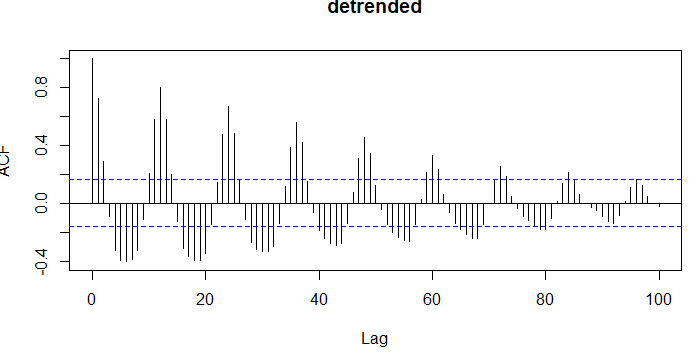
\includegraphics[width=5in]{img/detrended.PNG}

    \nl 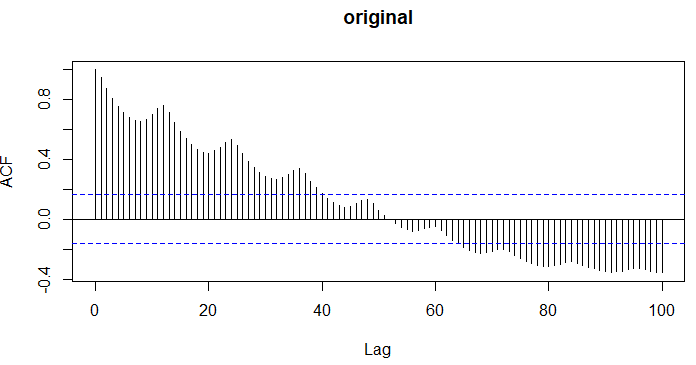
\includegraphics[width=5in]{img/original.PNG}

    \nnl In the detrended model, the residuals are decreasing in magnitude with time. In the original model, the residuals are simply decreasing with time. Thus the detrended model should converge to 0 but the original will diverge to $-\infty$

    \item Use \say{diff(airpass)} to compute the first difference of the original series. Examine its sample \textbf{acf} plot and compare it with the \textbf{acf} plot of the residuals in part (b)
    
    \nl \texttt{acf(diff(airpass), 100, main="1st diff")}\\
    \texttt{acf(resid(model), 100, main="detrended")}

    \nl The ACF plots look very similar between the two. The first diff seems to spikes with less magnitude that the detrended model, but not by much. The 1st difference also has more variance between its spikes, aka it's less smooth.
    \nl \notab{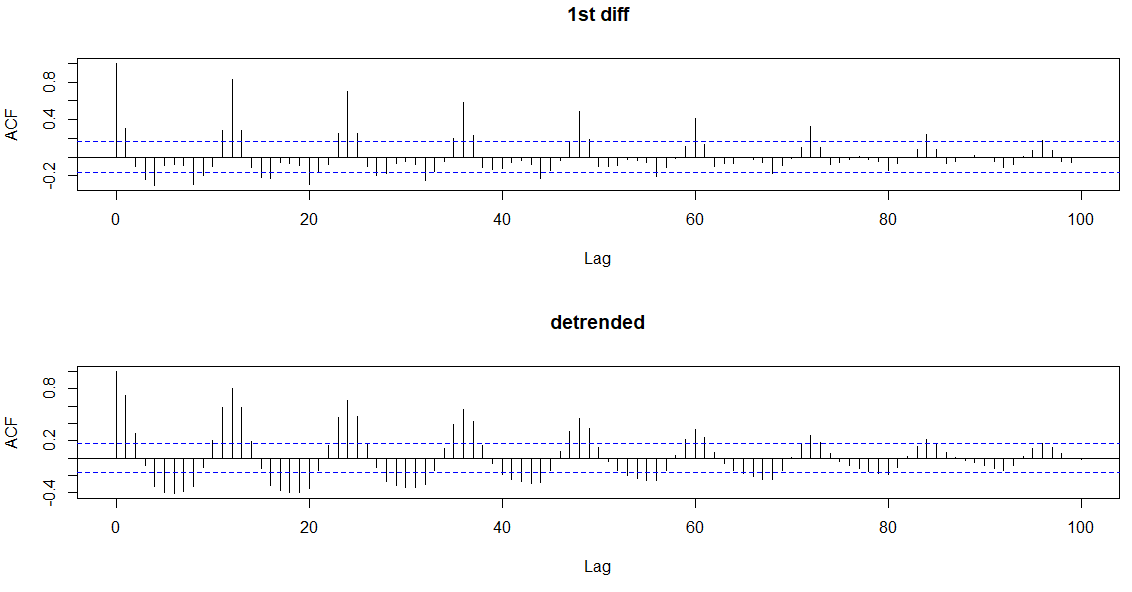
\includegraphics[width=7in]{img/7c.PNG}}
\end{enumerate}


\subsection{Exercise 2}
\textit{Show your work in order to earn credit.}

\nl 

Consider the model $x_t = w_t - 0.3 w_{t-1}$
\begin{enumerate}[label=(\alph*)]
    \item Find its ACVF (Autocovariance function).
    
    \nl \soln* $\Cov(x_s, x_t) = \Cov(w_s - 0.3w_{s-1}, w_t - 0.3w_{t-1})$. When $s = t$ then $\Cov(w_t, w_t) + \Cov(-0.3w_{t-1}, -0.3w_{t-1}) = 1.09 \sigma_w^2$. For $\abs{t-s} = 1$ then $\Cov(w_{t+1}-0.3w_{t+1-1}, w_t - 0.3w_{t-1}) = -0.3 \sigma_w^2$. Everything else is zero. That is, 
    $$\operatorname{ACVF} = \begin{cases}
        1.09 \sigma_w^2 & s=t\\ -0.3 \sigma_w^2 & \abs{s-t} = 1\\ 0 & \abs{s-t} \geq 2
    \end{cases}$$


    \item Find its ACF (Auto correlation function). 
    
    \nl \soln* Since $x_t$ is stationary ($\Eb{x_t} = 0$ and ACVF independent of $t$), then $$
        \operatorname{ACF} = \frac{\gamma(h)}{\gamma(0)}
        = \frac{\gamma(h)}{1.09 \sigma_w^2}.
    $$
    When $h=0$ $\gamma(0) = 1.09\sigma_w^2$, when $h=1$ $\gamma(1) = -0.3$, and when $h\geq 2$ $\gamma(h) = 0$. 
    Thus $$\operatorname{ACF} = \begin{cases}
        1 & h=0\\ -0.275 & \abs{h} = 1 \\ 0 & \abs{h} \geq 2
        \end{cases}$$
\end{enumerate}

\subsection{Exercise 3}
Identify the following models as ARMA$(p,q)$ models.
\begin{enumerate}[label=(\alph*)]
    \item $x_t = 0.5 x_{t-1} - 0.7 x_{t-2} + w_t - 0.3w_{t-1}\qquad$ ARMA$(2, 1)$
    \item $x_t + 0.6 x_{t-1} - 0.2x_{t-2} = w_t\qquad$ ARMA$(2, 0)$
    \item $x_t = w_t + 0.2w_{t-1}\qquad$ ARMA$(0, 1)$
\end{enumerate}



\end{document}
